\chapter{Implementácia}

\section{Metóda RISEI}

Metódu RISEI sme sa rozhodli implementovať v jazyku Python, keďže plánujeme používať knižnice pre strojové učenie akými sú \textit{tensorflow} či \textit{scikit-learn}.

\subsection{Generovanie masiek}

Na základe BPMN diagramu (Obr. \ref{fig:risei_diagram}) sme implementovali proces generovania masiek. Generovanie masiek prebieha paralelne vo viacerích procesoch použitím knižnice Python \textit{multiprocessing}. Metóda RISE pracuje s trojrozmernými dátami, avšak diagramy v tejto sekcii zobrazujú snímky a masky v 2D (konkrétne určitú vrstvu z 3D snímku) kvôli jednoduchšej vizualizácii. V tejto sekcii popíšeme jednotlivé kroky generovania masiek.

\paragraph{Vytvorenie náhodnej binárnej masky}

Náhodné binárne masky generujeme pomocou knižnice \textit{numpy}. Pomocou nasledovného kódu vygenerujeme $N$ náhodných masiek 3D binárnych matice. Obr. \label{fig:risei_inpainting_example} zobrazuje takúto binárnu maticu, ale v 2D. \textit{size} (veľkosť) a \textit{probability} (pravdepodobnosť) sú hyper-parametrami RISEI metódy. \textit{size} hovorí o veľkosti generovanej masky, čím je toto číslo väčšie tým bude výsledná maska viac fragmentovaná na malé plochy. \textit{probability} hovorí o tom, s akou pravdepodobnosťou daná plocha neprekrytá maskou. RISE používa predvolenú hodnotu \textit{size = 8}.

\begin{lstlisting}
    binary_masks = np.random.rand(N, size, size, size) < probability
\end{lstlisting}

\begin{figure}[h!]
    \centering
    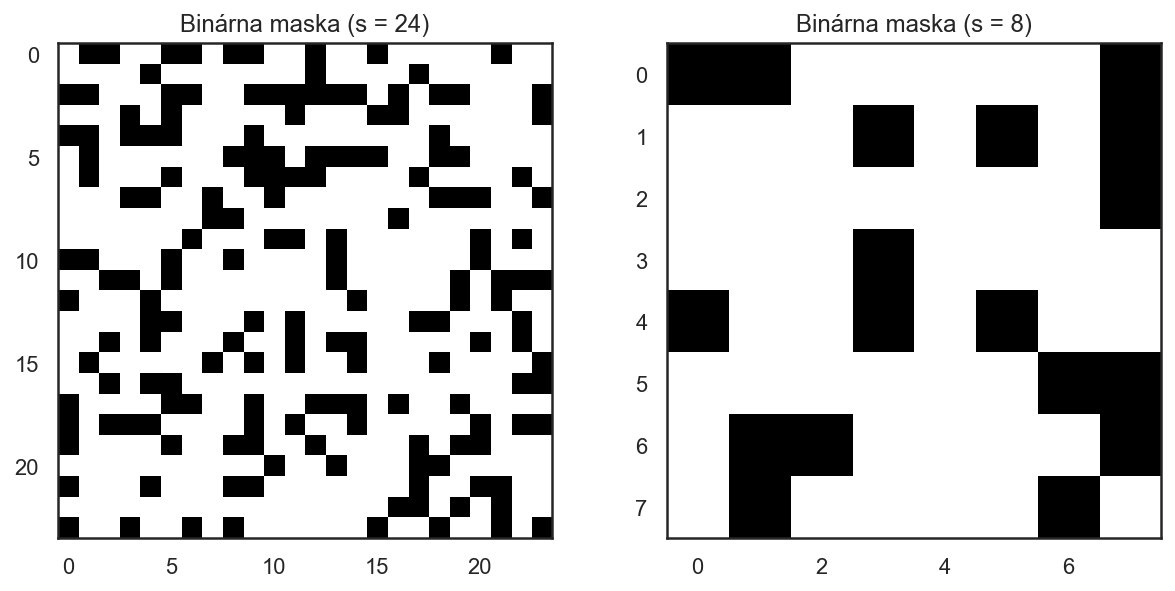
\includegraphics[width=13cm]{assets/images/binary_mask.png}
    \caption{Porovnanie dvoch binárnych masiek s rôznou veľkosťou (\textit{size}), čím väčšia veľkosť, tým je obrázok viac fragmentovaný.}
    \label{fig:binary_mask}
\end{figure}

\paragraph{Náhodné nastavenie pozície vyrezania, zväčšenie binárnej masky a orezenie na veľkosť obrázka}

Binárnu masku zväčšíme na veľkosť vstupného snímku plus menší offset (o veľkosti size). Následne zo zväčšenej masky na náhodnej pozícii vyrežeme masku o veľkosti vstupného snímku (Obr. \ref{fig:binary_mask_resized}). Táto maska určuje, ktoré miesta na snímku bude treba dokresliť - biele miesta, čiže jednotky. Tento krok v pôvodnej implementácii RISE nie je.

\begin{figure}[h!]
    \centering
    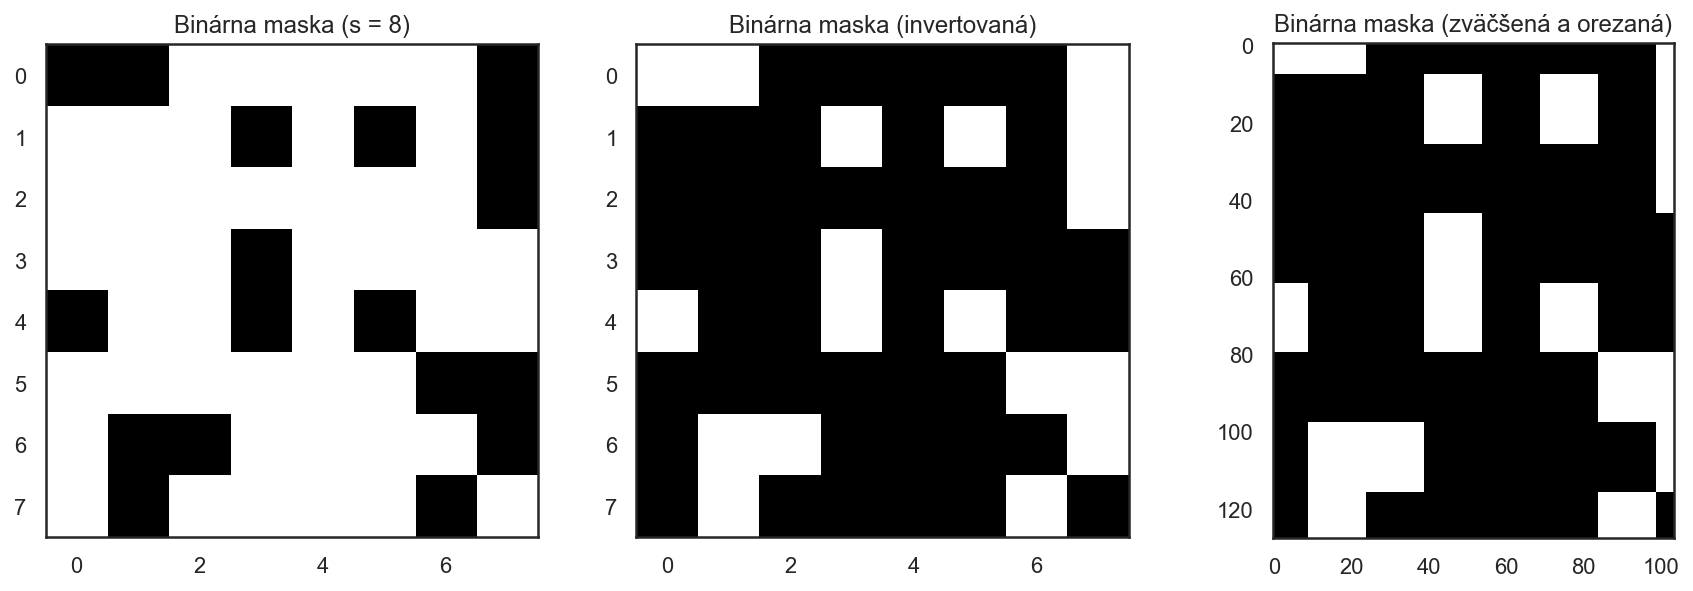
\includegraphics[width=13cm]{assets/images/binary_mask_resized.png}
    \caption{Vygenerovaná maska je zväčšená a orezaná na veľkosť vstupného snímku (ten je o veľkosti $[104, 128, 104]$ pričim na obrázkoch je vizualizovaná druhá a tretia dimenzia). Úplne vľavo je binárna maska o veľkosti $8$. V strede je invertovaná binárna maska (kvôli ďaľšiemu pracovanou s ňou) a vpravo je orezaná binárna maska o veľkosti vstupného snímku.}
    \label{fig:binary_mask_resized}
\end{figure}

\paragraph{Zväčšenie pomocou bilineárnej interpolácie a orezanie masky na veľkosť obrázka}

Tak ako v poôvodnej implementácii RISE, vytvoríme ''čiernu'' masku na zakrytie častí obrázku. Pôvodnú binárnu masku pomocou bilineárnej interpolácie (funkcia \textit{resize} z knižnice \textit{scikit-learn}) zväčšíme na veľkost vstupného snímku plus menší offset, následne vyrežeme na náhodnej pozicii masku o veľkosti vstupného snímku (táto náhodná pozícia je rovnaká ako pri orezávani binárnej masky bez interpolácie, preto je v BPMN diagrame v samostatnom kroku).

\begin{figure}[h!]
    \centering
    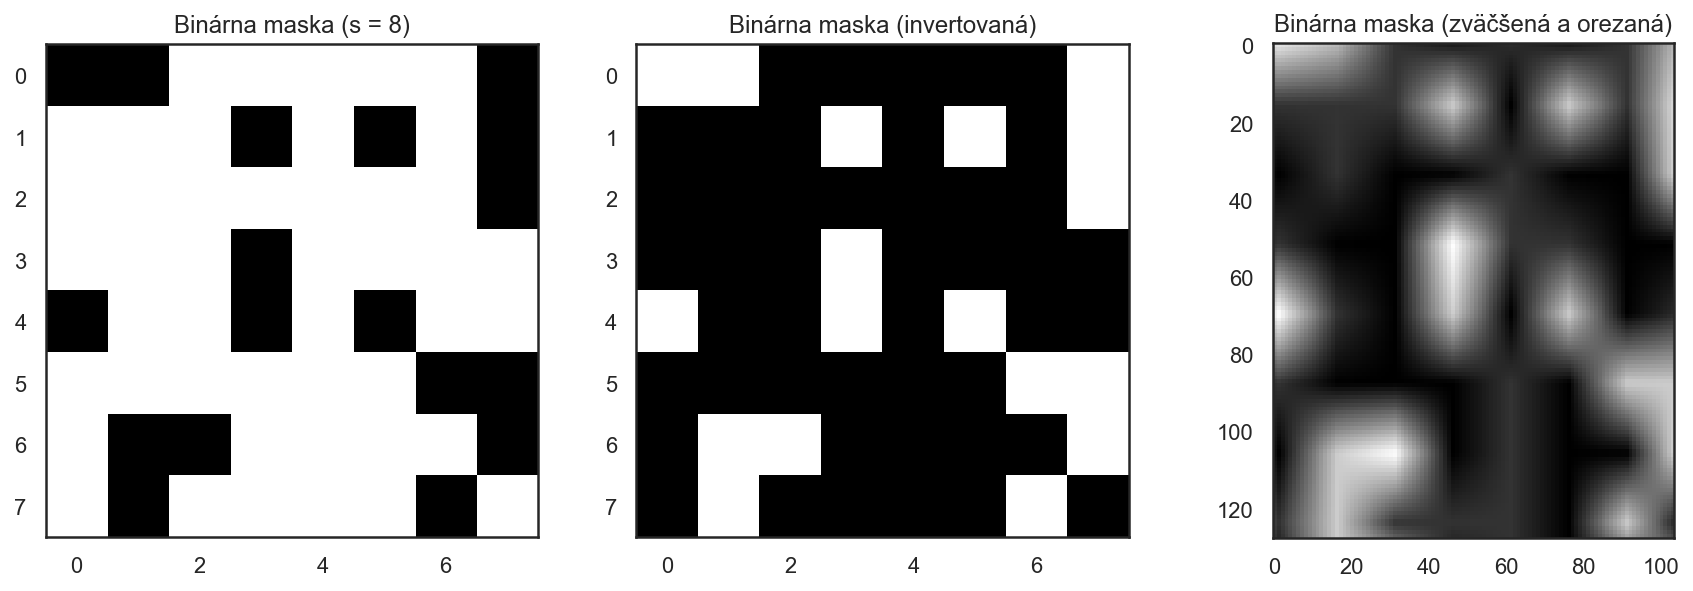
\includegraphics[width=13cm]{assets/images/interpolated_mask.png}
    \caption{Vygenerovaná maska je zväčšená pomocou bilineárnej interpolácie a orezaná na veľkosť vstupného snímku (ten je o veľkosti $[104, 128, 104]$ pričim na obrázkoch je vizualizovaná druhá a tretia dimenzia). Úplne vľavo je binárna maska o veľkosti $8$. V strede je invertovaná binárna maska (kvôli ďaľšiemu pracovanou s ňou) a vpravo je orezaná interpolovaná ''čierna'' maska o veľkosti vstupného snímku.}
    \label{fig:interpolated_mask}
\end{figure}

\paragraph{Prekrytie masky s obrázkom a dokreslenie zamaskovaných častí obrázka}

Keďže pracujeme nad trojrozmernými dátami, pokúsili sme sa použiť dokreslovanie obrázka v 3D. Na to sme sa pokúsili použiť funkciu \textit{inpaint} s knižnice \textit{scikit-image}, avšak dokreslenie jednej masky bolo veľmi časovo náročné (trvanie bolo až v minútach kde dokreslenie v 2D je v sekundách) a my ich potrebujeme generovať tisíce, preto sme trojrozmerného dokreslovania upustili.

Dokreslovanie dvojrozmerných snímkov z 3D snímku má avšak svoje nevýhody. Nech máme snímky o veľkosti $[z, y, x]$, pri 2D dokreslení musíme dokreslovať $z$ snímkov o veľkosti $[y, x]$ (alebo $y$ snímkov o veľkosti $[y, x]$, alebo $x$ snímkov o veľkosti $[y, z]$). Pri takomto dokreslovaní, dokreslenie z pohľadu $[y, x]$ vyzerajá byť správne, avšak z iného pohľadu, napr. $[z, x]$ sa javí byť dokreslenie nesprávne, najmä kvôli vzniknutým ostrím hranám (Obr. \ref{fig:inpaint_3x_2d}). Toto sme sa pokúsili obýsť tak, že dokreslujeme zo všetkých troch pohľadov a robíme priemer pre každý voxel zo všetkých troch dokreslení. Takto je výsledok o niečo lepší, tj. z každej strany je dokreslenie lepšie ako nesprávne dokreslenie z 2D ale o niečo horšie ako správne dokreslenie z 2D. Na označenie miest, ktoré treba dokresliť sme použili zväčšenú binárnu masku (Obr. \ref{fig:binary_mask_resized}). Dokreslenie vykonávame funkciou \textit{inpaint} z knižnice \textit{cv2 (Open CV)}. Používame dokreslovací algoritmus \textit{cv2.INPAINT\_TELEA}, keďže pomocou neho sme dosahovali vizuálne najlepšie výsledky. Funkcia \textit{cv2.inpaint} vyžaduje ako parameter \textit{inpaint\_radius} (Obr. \ref{fig:inpaint_radius}), čo je jedným z hyper parametrov našej metódy.

\begin{figure}[h!]
    \centering
    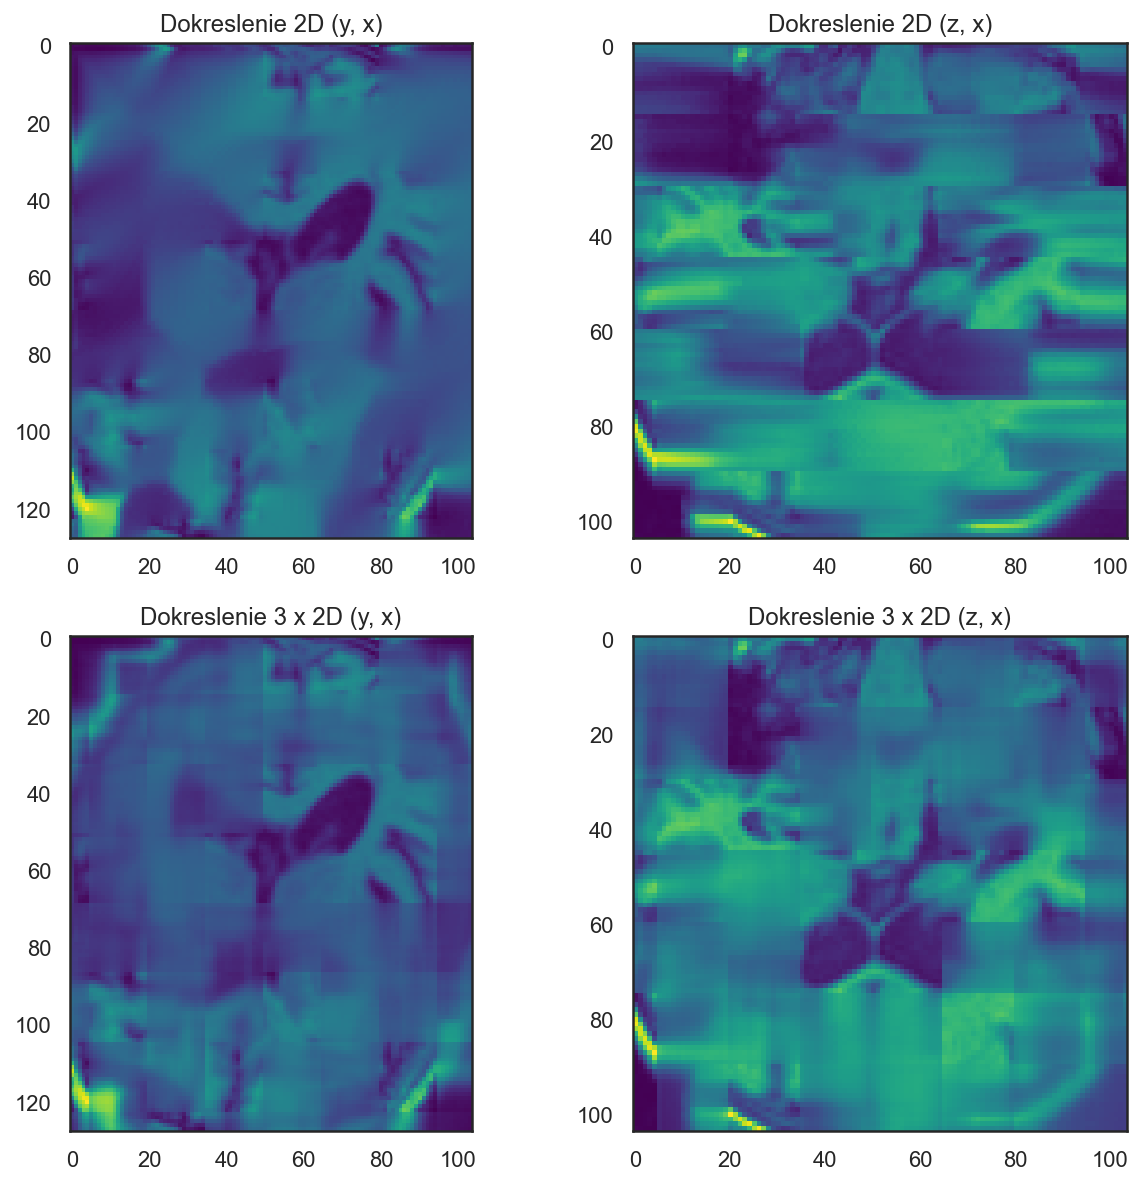
\includegraphics[width=13cm]{assets/images/inpaint_3x_2d.png}
    \caption{Porovnanie 2D dokreslenia (iba v jednej dimenzii) a spriemerovaného 3x 2D dokreslenia (v každej dimenzii). Použitie iba 2D dokreslenia je kvalitné iba v jednej dimenzii a v ostatných je deštruktívne - vytvára ostré hrany. Použitie 3x 2D dokreslenia a spriemerovanie pre každý voxel produkuje celkom dobré dokreslenia po všetkých dimenziách.}
    \label{fig:inpaint_3x_2d}
\end{figure}

Keďže sa pôvodná implementácia RISE prekrýva miesta tak, aby nevznikali ostré hrany medzi zakrytím miestom a pôvodným obrázkon, a teda vznikol plynulý prechod, aj pri dokreslení vytvárame plynulý prechod medzi dokreslením a pôvodným obrázkom (Obr. \ref{fig:inpaint_soft_corners}). Tento prechod je implementovaný nasledovne.
\begin{lstlisting}
    # binary_mask int[z, x, y] - upsized binary mask
    # image float[z, x, y] - original image
    # mask float[z, x, i] - upsizded and interpolated binary mask
    # inpaint_radius int
    inpainted = cv.inpaint(image, binary_mask, inpaint_radius, cv2.INPAINT_TELEA)
    inpainted_blend = image * mask + inpainted * (1 - mask)
\end{lstlisting}

\begin{figure}[h!]
    \centering
    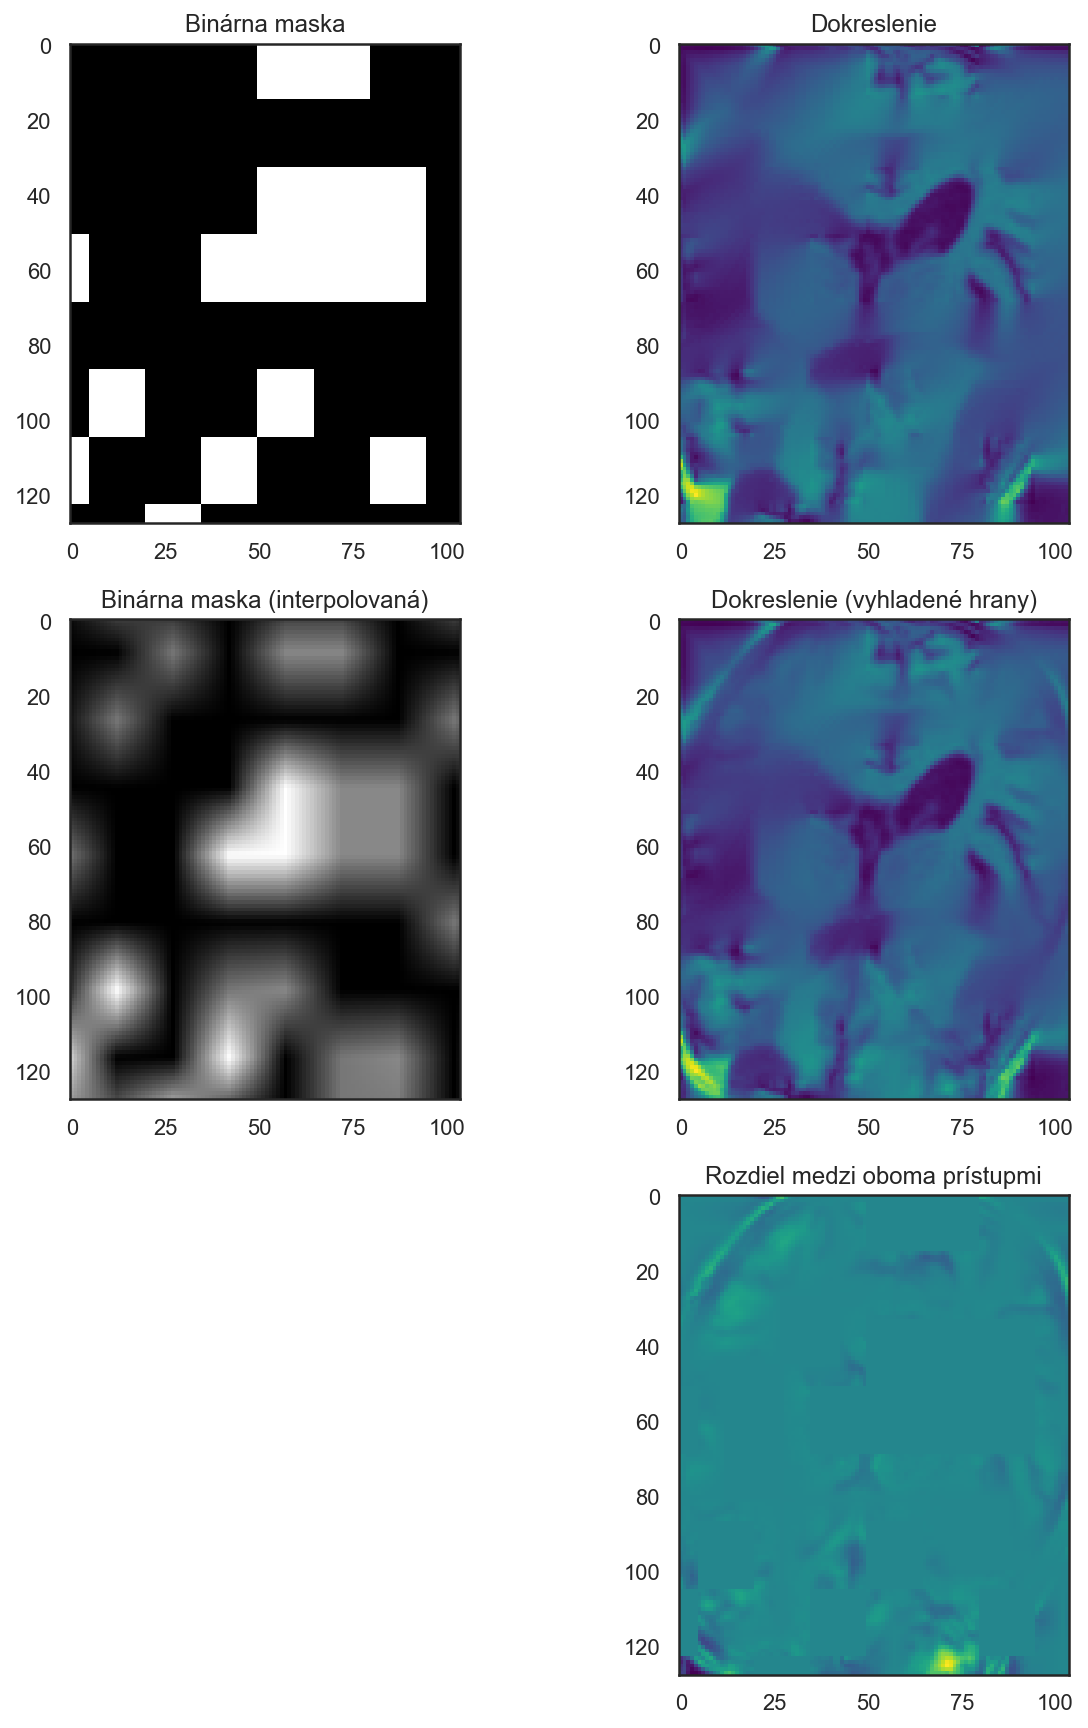
\includegraphics[width=10cm]{assets/images/inpaint_soft_corners.png}
    \caption{Príklad vyhladzovania hrán dokreslenia - splynutie dokreslenia s pôvodným snímkom (štvrtý snímok). Druhý snímok zobrazuje ostré hrany po dokreslení - bez splývania s obrázkom. Piaty snímok zobrazuje rozdiel medzi oboma prístupmi. Môžeme si všimnúť, že na obrázku sí viditeľné miesta, kde sa nachádza prechod na interpolovanej binárnej maske. O tieto miesta (informácie) je dokreslenie s vyhladenými hranami ''bohatšie''.}
    \label{fig:inpaint_soft_corners}
\end{figure}

\begin{figure}[h!]
    \centering
    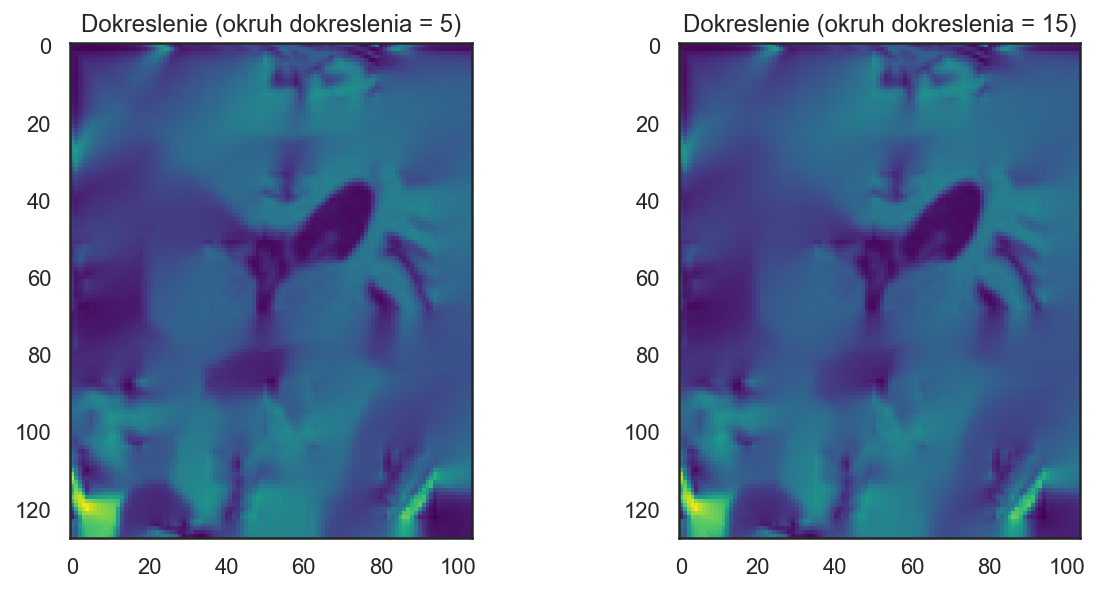
\includegraphics[width=13cm]{assets/images/inpaint_radius.png}
    \caption{Porovnanie okruhov dokreslenia (parameter \textit{inpaint\_radius}), rozdiel vo výsledku nie je veľmi viditelný, avšak s väčśím oruhom dokreslenia je generovanie rádovo pomalšie. (pri generovaní bolo vypnuté splynutie dokreslenia so snímkom aby bol rozdiel aspoň trochu viditeľný)}
    \label{fig:inpaint_radius}
\end{figure}

\paragraph{Prekrytie dokreslenej masky a čiernej masky s obrázkom}

Keďže prekrývam tri rôzne vrstvy - originálny snímok, čiernu masku a dokreslený snímok môžem tieto vrstvy skombinovať v rôznom pomere a tým vytvoriť nový obrázok.

Toto som implementoval zavedením parametrov $b1$ a $b2$ (skratka od slova prechod, angl. blend), ktoré hovoria o pomere medzi originálnym snímkom a dokresleným snímkom, a originálnym snímkom spojeným s dokreslením a čiernou maskou (Obr. \ref{fig:risei_layers}). Pri týchto parametroch platí, že $0 <= b1, b2 <= 1$. Takto zadefinované parametre mi umožňujú vytvoriť zakaskovaný snímok iba s čiernou maskou ($b1 = 0$, $b2 = 1$) či iba s dokreslením ($b1 = 1$, $b2 = 0$).

\begin{figure}[h!]
    \centering
    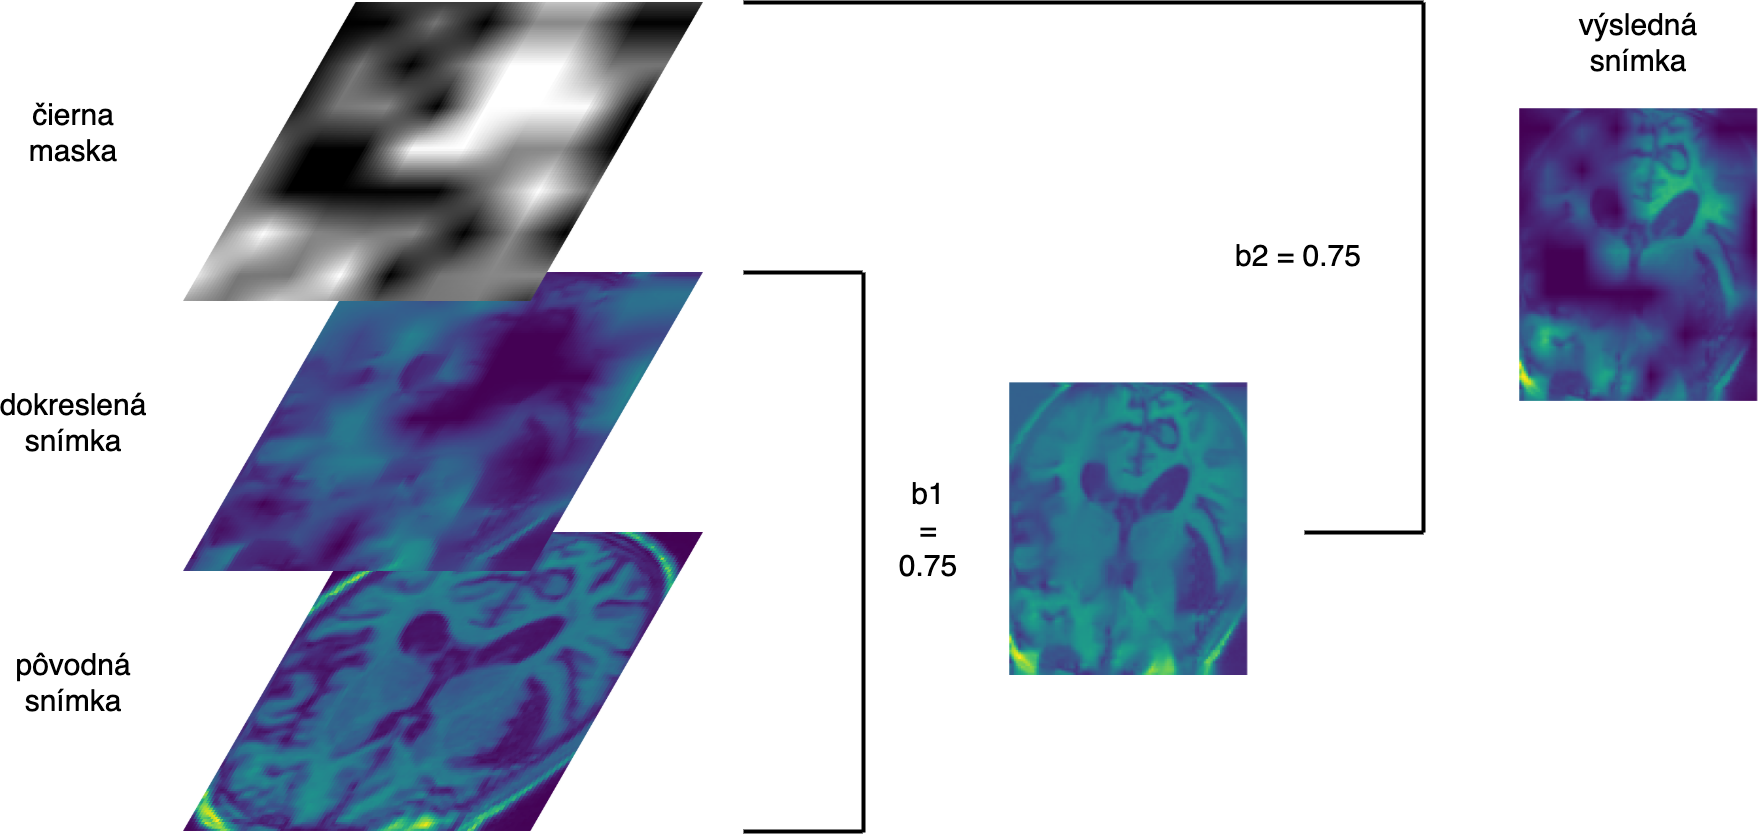
\includegraphics[width=13cm]{assets/images/risei_layers.png}
    \caption{Príklad, ako vyzerá spojenie originálneho snímku, dokresleného snímku a čiernej masky. V diagrame je zobrazený aj výsledok medzikroku spojenia dokresleného snímku a pôvodného snímku. Parametre boli nastavené na $b1 = 0.75$ a $b2 = 0.75$.}
    \label{fig:risei_layers}
\end{figure}

Názov ''čierna'' maska pochádza z pôvodnej implementácie RISE, kde sa obrázok prekrýval čiernou maskou. V našej implementácii neprekrývame farbou, ale hodnotou, tj. ''čierna'' je hodnota $0$ (minimum). Okrem použitia hodnoty $0$, môžeme použiť aj $1$, \textit{priemer} či \textit{medián} (toto je ďaľším hyper-parametrom našej metódy). Zjednodušená (a menej efektívna, v produkčej implementácii sa niektoré inštrukcie nevykonávajú keď \textit{b1} je 0 alebo \textit{b2} je 0) implementácia spojenia jednitlivých vrstiev vyzerá nasledovne.

\begin{lstlisting}
    # image float[z, x, y] - original image
    # inpainted_blend float[z, x, y] - inpainted image
    # mask float[z, x, i] - upsizded and interpolated binary mask
    # b1 float <0, 1>
    # b2 float <0, 1>
    # b2_value string - what value use in "black" mask (min/max/mean/median)

    # merge with inpainted image
    new_image = (1 - b1) * original_image + b1 * inpainted_blend

    value = 0 # black
    if b2_value == 'max':
        value = 1 # white
    elif b2_value == 'mean':
        value = np.mean(original_image)
    elif b2_value == 'median':
        value = np.median(original_image)
    # merge with "black" mask
    new_image = b2 * mask * new_image + (b2 * (1 - mask) * value)
\end{lstlisting}

Kompletný zoznam parametrov metódy RISEI sa nachádza v tabuľke \ref{tab:risei_params}.

\begin{table}[]
    \begin{tabular}{p{0.25\linewidth} | p{0.15\linewidth} | p{0.5\linewidth}}
        \hline
        Názov             & Dátový typ & Popis                                                               \\ \hline
        s                 & int        & Veľkosť strany binárnej 3D matice.                                        \\
        p                 & float      & Pravdepodobnosť, že plocha nebude prekrytá maskou.                        \\
        b1                & float      & Miera prekrytia medzi originálnym snímkom a dokresleným snímkom.          \\
        b2                & float      & Miera prekrytia s ''čiernou'' maskou.                                     \\
        b2\_value         & string     & Hodnota ''čiernej'' masky, môže to byť minimum, maximum, medián, priemer. \\
        in\_paint\_radius & float      & Polomer dokreslenia algoritmom z knižnice OpenCV.                         \\ \hline
    \end{tabular}
    \caption{Zoznam parametrov metódy RISEI.}
    \label{tab:risei_params}
\end{table}

\subsection{Vytvorenie tepelných máp}

Na základe návrhu (Sekcia \ref{sec:risei}) sme implementovali vytváranie tepelných máp. Keďže generovanie tepelnej mapy si vyžaduje vygenerovať veľký počet zamaskovaných snímkov, ktoré v istom momente musia byť všetky uložené v pamäti, generujeme a vyhodnocujeme zamaskované snímky v dávkach (angl. batch). Zdrojový kód nižšie, implementuje vytvorenie jednej tepelnej mapy. Príklad vytvorenej tepelnej mapy uvádzame na obrázku \ref{fig:heatmap_example}.

\begin{lstlisting}
# image_x float[z, x, y, 1] - original image
# masks_count int - how many masks are generated to create a heatmap
# batch_size - how many masks to evaluate on model
# risei_batch_size int - how many masks to generate in one batch
# seed int int - seed for mask generation
# cls_idx int - index of target class in model output vector
# model tf.keras.Model - instance of tensorflow model

risei = RISEI(s=8, p=0.5, b1=0.5, b2=0.5, b2_value='median', in_paint_radius=5)
heatmap = np.zeros(shape=image_x.shape[:3])
batch_count = math.ceil(masks_count / risei_batch_size)
weights = 0

for batch_idx in range(batch_count):
    batch_masks_count = min(risei_batch_size, masks_count - batch_idx * risei_batch_size)
    # reshape input for RISEI since it works with [z, y, x] shape
    # batch_x float[z, x, y] - images to evaluate with masks already applied
    # masks float[z, x, y] - interpolated binary masks (so we know which places we inpainted or masked)
    batch_x, masks = risei.generate_masks(batch_masks_count, image_x.reshape(image_x.shape[:3]), seed=seed)
    y_pred_batch_x = model.predict(batch_x.reshape((-1, *image_x.shape)), batch_size=batch_size)

    for mask, y_pred in zip(masks, y_pred_batch_x):
        # invert the mask, since 1 is for no masking
        # y_pred is the activation for the input masked image on last layer (softmax)
        heatmap = heatmap + y_pred[cls_idx] * (1 - mask)
        weights += y_pred[cls_idx]

heatmap = heatmap / weights
\end{lstlisting}

\begin{figure}[h!]
    \centering
    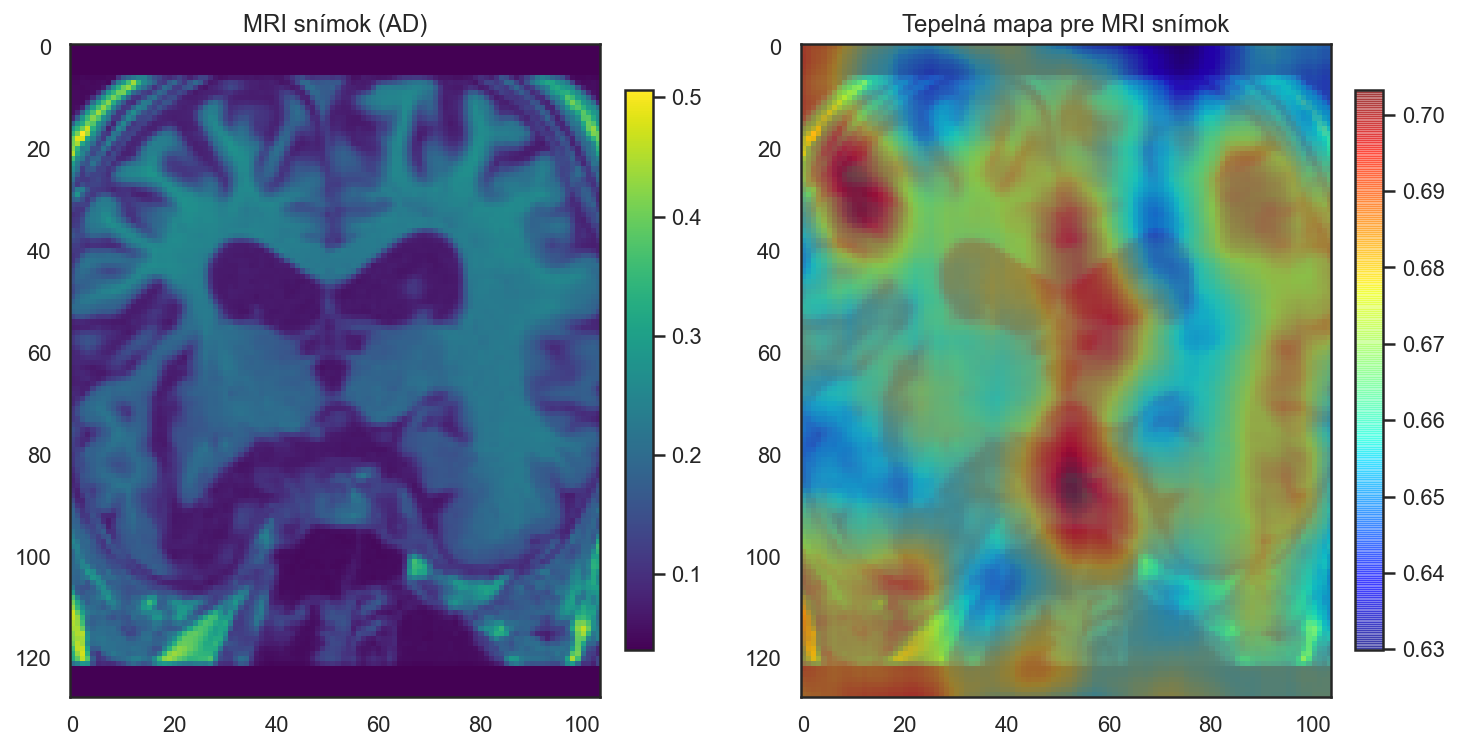
\includegraphics[width=10cm]{assets/images/heatmap_example.png}
    \caption{Príklad vytvorenej tepelnej mapy (vpravo) k MRI snímku (vľavo). Mierka vujadruje priemernú mieru aktivácie pre daný voxel.}
    \label{fig:heatmap_example}
\end{figure}

\subsection{Vyhodnotenie tepelných máp}

Zatiaľ sme implementovali, podľa návrhu riešenia (Sekcia \ref{sec:evaluation_design_method_quality}), iba metriky \textit{insertion} a \textit{deletion}.

\subsubsection{Metriky insertion \& deletion \label{sec:insertion_deletion}}

Tieto metriky fungujú tak, že postupne odstraňujeme/pridávame pixely z obrázku a tieto obrázky vkladáme do modelu a zaznamenávame si aktiváciu na poslednej vrstve pre predikovanú triedu. V prípade obrázkov, a teda dvojrozmerných dát je to ešte výpočtovo zvládnutelné, avšak v prípade trojdimenzionálnych rádiologických simkov to už môže byť problém. Naše vstupné snímky majú po zmenšení rozmer \textit{[104, 128, 104]}, čiže ak aby sme odstraňovali zo snímku po jednom voxeli, museli by sme vykonať \textit{1 384 448} evaluácii pomocou nášho modelu (čo trvá niekoľko hodín, aj pri evaluovaní v maximálnych možných dávkach vzhľadom na pamäť grafickej karty). Preto sme sa rozhodli, že budeme pridávať po $n$ (~100) voxeloch v každom kroku. V prípade metódy insertion vkladáme do snímku plného núl (môžeme prípadne aj jednotiek). Keďže kód je rozsiahlejší, uvedieme len pseudokód.

\begin{lstlisting}
method = 'insertion'
step_size = 150 # how many voxels to insert/delete in one evaluation
image_x, image_y = get_image()
image_y_pred = model.predict(image_x)
heatmap = get_heatmap()
voxels = get_ordered_voxels_by_heat(heatmaps)
sequence = get_images_sequence(voxels, step_size) # create a sequence from images where each next image has n inserted/deleted voxels
y_pred = []

for batch_x, batch_y in sequence:
    batch_y_pred = model.predict(batch_x)
    for y in batch_y_pred:
        y_pred.append(y)

auc = metrics.auc([i * step_size for i in range(len(y_pred))], y_pred) / get_voxels_count(image_x)
\end{lstlisting}

\section{Model na detekciu Alzheimerovej choroby na základe MRI snímkov}

V tejto sekcii popíšem impelentáciu, z ktorého predikcií budeme vytvárať tepelné mapy. Náš model - neuónovú sieť sme sa rozdhodli implementovať v knižnici Tensorflow (v2.3.0). Naším cieľom nie je natrénovať najlepší model na dekekciu Alzheimerovej choroby, ale model ktorý je použiteľný na overenie nami narvhnutej metódy. Preto nevykonáme komplexnejšie prístupy k detekcii Alzheimerovej chorby, ktoré sme popísali v analýze (Sekcia \ref{sec:nn_ad_prediction}), ako je napríklad učenie prenosom pomocou autoenkodéra.

\subsection{Dátová sada}

Použili sme dátovú sadu ADNI. Ako vstup modelu je celý MRI snímok (tj. všetky tri dimenzie), nepoužívame žiadné ine údaje z dátovej sady ADNI, ako napríklad demografické údaje a pod. keďže model plánujeme používať iba na vytváranie tepelných máp pre vstupné snímky. 

V dátovej sade sa nachádza celkom 502 MRI snímkov, z toho 311 pacientov s Alzheimerovou chorobou (AD) a 191 bez (CN). Dátovú sadu máme teda nevyváženú a model môže začať preferovať jednu triedu. Na predíjdenie tomuto javu existuje niekoľko techník, napríklad nadvzorkovanie (angl. oversampling) alebo podvzorkovanie (angl. undersampling) kedy sa doplní synetetickými minoritná trieda, alebo sa odstránia nejaké pozorovania z majoritnej triedy. My sme sa však rozhodli nastaviť predikovaným triedam váhy, ktoré sú zohladnené v chybovej funkcii, taktiež sme nainicializovali chybu \footnote{\url{https://www.tensorflow.org/tutorials/structured\_data/imbalanced\_data\#optional\_set\_the\_correct\_initial\_bias}} pre neuróny na poslednej vrstve aby reflektovala to, že triedy sú nevyvážené.

Dátovú sadu sme náhodným výberom rozdelili na trénovaciu a testovaciu v pomere 80/20. Validačnú sadu sme nerobili, pretože máme málo dát a neplánujeme robiť veľké hľadania optimálnych hyper-parametrov. V budúcnosti možno zvážime vykonanies krížovej validácie (angl. cross validation) pri trénovaní. Aj po rozdelení sa nám podarilo zachovať pôvodný pomer medzi triedami -- 62/38 (Obr. \ref{fig:dataset_classes}).

\begin{figure}[h!]
    \centering
    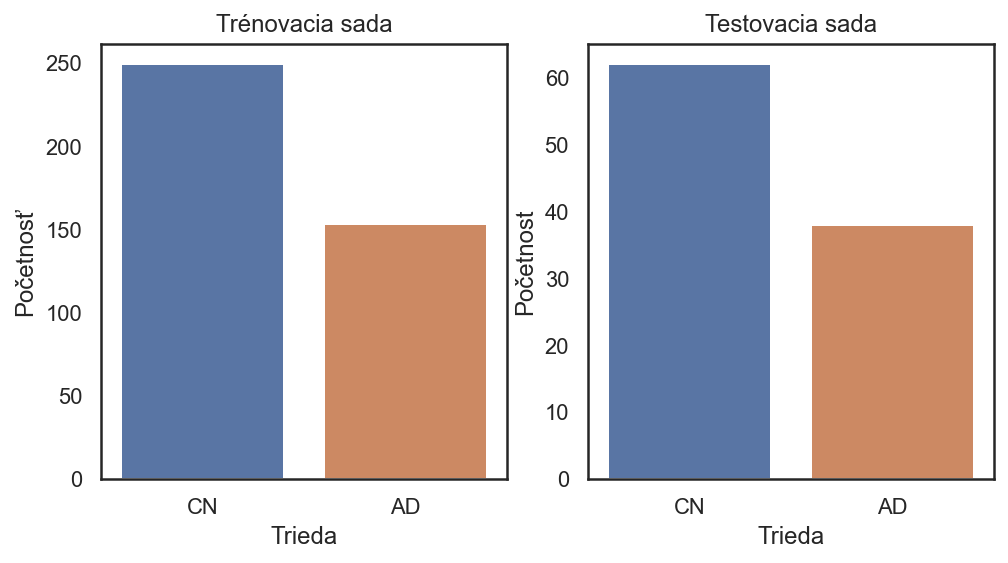
\includegraphics[width=10cm]{assets/images/dataset_classes.png}
    \caption{Početnosť tried medzi trénovacou a testovacou sadou - je zrejmá prevaha triedy AD.}
    \label{fig:dataset_classes}
\end{figure}

\subsubsection{Predspracovanie}

MRI snímky boli predspracované štandardnou postupnosťou nástroja freesurfer, avšak nevykonali sme odstránenie lebky z MRI snímkov.
Okrem iného sme vykonali:

\begin{itemize}
    \item Upravenie vstupných snímkov na rovnakú veľkosť 104 x 128 x 104 voxelov. \citeauthor*{esmaeilzadeh2018end} upravili vstupné snímky na veľkosť 116 x 130 x 83, k týmto číslam sme sa pokúsili priblížiť. Pomer veľkostí dimenzií ale nemáme rovnaký, aj z dôvodu, že sme nevykonali odstránenie lebky zo vstupných snímkov.
    \item Štandardizáciu vstupných dát (preškálovanie na rozsah $<0, 1>$) nasledovným vzorcom: $\frac{(image\_x - images\_min])}{(images\_max - images\_min)}$.
\end{itemize}

\subsubsection{Augmentácie}

Keďže máme málo dát, rozhodli sme sa dáta augmentovať (Obr. \ref{fig:augmentations}). Dáta náhodne augmentujeme v každej dávke (angl. batch). Implementovali sme nasledovné augmentácie:

\begin{itemize}
    \item Vymenenie hemisfér mozgu (\citeauthor*{esmaeilzadeh2018end}) s pravdepodobnosťou 50\%
    \item Náhodná rotácia o 0 až 5 stupňov s pravdepodobnosťou 20\%
    \item Náhodné priblíženie do 80\% veľkosti snímku s pravdepodobnosťou 20\%
    \item Náhodné gaussovské rozmazanie (max $sigma = <0.85, 1>$) s pravdepodobnosťou 20\%
    \item Náhodný gaussovský šum pravdepodobnosťou 20\%
\end{itemize}

\begin{figure}[h!]
    \centering
    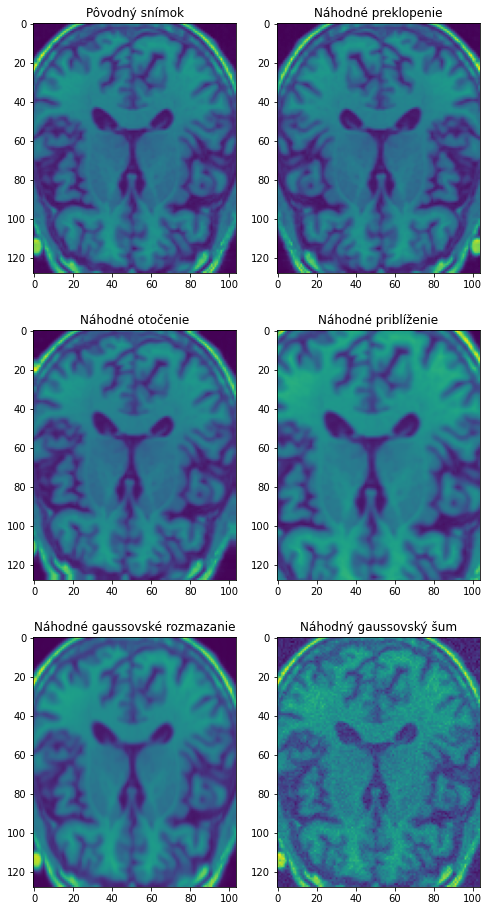
\includegraphics[width=10cm]{assets/images/augmentations.png}
    \caption{Príklady aplikácie implementovaných augmentácií.}
    \label{fig:augmentations}
\end{figure}

\subsection{Model}

Rozhodli sme sa implementovať a porovnať niekoľko architektúr neurónových sietí.

\paragraph{3D konvolučná neurónová sieť od \citeauthor*{esmaeilzadeh2018end}} Túto neurónovú sieť sme sa rozhodli implementovať, pretože jej autori pomocou nej dosiahli veľmi slušné výsledky (94.1\% presnosť). Implementovali sme jednoduchšiu verziu, ktorá dosahovala lepšie výsledky, opísali sme ju v sekcii \ref{sec:nn_ad_prediction}. Táto neurónová sieť ma celkovo \textit{2 899 778} parametrov.

\paragraph{2D ResNet a 3D ResNet} Keďže reziduálne neúronové siete dosahujú pri klasifikačných úlohách nad obrazovými dátami veľmi dobre výsledky vyskúšame aj tieto architektúry. V prípade 2D ResNetu-u používame 2D konvolúcie, tie nám budú fungovať aj napriek tomu, že máme 3D dáta. Vstup do 2D ResNet-u je tiež 3D matica, ktorej tretia dimenzia býva o obvykle o dĺžky 1 alebo 3 (RGB), v našom prípade bude o veľkosti poslednej dimenzie snímku. Rozmery vstupných dát pre 2D ResNet budú $[104, 128, 104]$ a pre 3D ResNet $[104, 128, 104, 1]$. Za konvolučné vrstvy a globálnu združovaciu vrstvu sme pripojili dve plne prepojené vrstvy s 512, 256 a 128 neurónami a aktiváciou \textit{ReLU}, následne už nasleduje iba posledná vrstva s aktiváciou \textit{softmax}. Tieto neurónové siete majú celkovo \textit{12 689 602}, resp. \textit{34 356 354} parametrov.

Do neurónových sietí sme ešte pridali dropout a dávkovú normalizáciu (angl. batch normalization). Dropout sme pridali pred plne prepojené vrstvy. Dávkovú normalizáciu sme pirdali v konvolučných vrstvách pred aplikovaním nelinearity, tak ako je to odporučené od \citeauthor*{ioffe2015batch} v \textit{Batch Normalization: Accelerating Deep Network Training by Reducing Internal Covariate Shift}. Na poslednej vrstve sa nachádzajú dva neuróny s aktiváciou \textit{softmax}.

\subsection{Trénovanie}

Pri trénovaní sme použili:

\begin{itemize}
    \item kategorickú entropiu (angl. categorical crossentropy) ako chybovú funkciu s podporou pre nevyvážené triedy (tj. táto funkcia brala ohľad na váhy tried, ktoré sme nastavili),
    \item optimizér Adam s prevolenými nastaveniami,
    \item exponenciálne tlmenie rýchlosti učenia (angl. learning rate decay), $0,96$ každých 25 epoch
    \item skoré zastavenie trénovania ak sa metrika AUC (plocha pod krivkou) nezlepšila za posledných 50 epoch,
    \item veľkosť dávky (angl. batch size) -- 10 (vždy tak, aby sme naplno využili pamäť grafickej karty),
    \item $l2$ regularizáciu (rovnako ako \citeauthor*{esmaeilzadeh2018end}).
\end{itemize}

Trénovali sme iteratívne, začali sme obyčajným modelom a postupne sme pridávali augmentácie, dávkovú normalizáciu, dropout a regularizáciu pričim sme postupne dolaďovali parametre. Najlepšie výsledky sme dosiahli s architektúrou 3D ResNet s presnosťou 80\% (Tabuľka \ref{tab:model_training_results}). Nepodarilo sa nám nám teda priblížiť k výsledkom analyzovaných prác.

\begin{landscape}
    \begin{table}[]
        \centering
        \begin{tabular}{l|rrr|rrr|rrr|}
            \cline{2-10}
            \multirow{2}{*}{}    & \multicolumn{3}{c|}{3D CNN} & \multicolumn{3}{c|}{3D ResNet} & \multicolumn{3}{c|}{2D ResNet} \\ \cline{2-10} 
            &
            \multicolumn{1}{c|}{Acc.} &
            \multicolumn{1}{c|}{Sens.} &
            \multicolumn{1}{c|}{Spec.} &
            \multicolumn{1}{c|}{Acc.} &
            \multicolumn{1}{c|}{Sens.} &
            \multicolumn{1}{c|}{Spec.} &
            \multicolumn{1}{c|}{Acc.} &
            \multicolumn{1}{c|}{Sens.} &
            \multicolumn{1}{c|}{Spec} \\ \hline
            \multicolumn{1}{|l|}{Baseline}             & 0.71    & 0.76    & 0.63    & 0.71     & 0.79     & 0.57     & 0.67     & 0.77     & 0.50     \\
            \multicolumn{1}{|l|}{+ Augmentácie}        & 0.67    & 0.68    & 0.66    & 0.69     & 0.84     & 0.45     & 0.76     & 0.90     & 0.52     \\
            \multicolumn{1}{|l|}{+ Batch Norm}         & 0.75    & 0.77    & 0.71    & 0.80     & 0.85     & 0.71     & 0.77     & 0.89     & 0.58     \\
            \multicolumn{1}{|l|}{+ Dropout}            & 0.75    & 0.76    & 0.74    & 0.74     & 0.94     & 0.42     & 0.77     & 0.85     & 0.63     \\
            \multicolumn{1}{|l|}{+ Regularizácia (l2)} & 0.71    & 0.70    & 0.71    & 0.79     & 0.87     & 0.66     & 0.78     & 0.89     & 0.61    
        \end{tabular}
        \caption{\textbf{Výsledky trénovania.} Acc. = presnosť (angl. Accouracy), Sens. = senzitivita (angl. Sensitivity), Spec. = Špecificita (angl. Specificity)}
        \label{tab:model_training_results}
    \end{table}
\end{landscape}

Oproti \citeauthor*{esmaeilzadeh2018end}, ktorí dosiahli presnosť až 94\%, sme dosiahli presnosť len 72\% avšak sme mali menej dát (o 339 pozorovaní menej), neodstraňovali sme zo snímkov lebku a nepoužili sme pri klasifikácii vek pacienta. Avšak robili sme viac augmentácií, a po ich pridaní sa úspešnosť modelu zhoršila (Obr. \ref{fig:3d_cnn_training}) (ale následne sa už iba zlepšovala), je teda možné, že niektoré augmentácie sú nekorektné a deštruktívne. V ďaľších experimentoch by sme mali pridávať augmentácie po jednej. Aj po pridaní veľmi slabej regularizácie, sa úspešnosť modelu zhoršila. V prípade 2D a 3D ResNet architektúr sa nám podarilo dosiahnuť lepšie výsledky, avšak v ich prípade sa sieť neskôr začala pretrénovávať (Obr. \label{ref:2d_3d_res_net_training}
) aj napriek použitej regularizácii, čo môže naznačovať, že sú tieto architektúry na náš problém príliš komplexné.

Možné vylepšenia (zoradené podľa subjektívneho pomeru úsilie/vplyv):
\begin{itemize}
    \item Pridávať augmentácie postupne a vyhodiť tie deštruktívne.
    \item Menej ''agresívne'' augmentácie.
    \item Odstránenie lebky zo snímkov.
    \item Nájsť a použiť viac dát.
    \item Krížová validácia v prípade väčšieho nastavovania hyperparametrov.
    \item Učenie prenosom pomocou autoenkodéra \cite{hosseini2016alzheimer}.
\end{itemize}

\begin{figure}[h!]
    \centering
    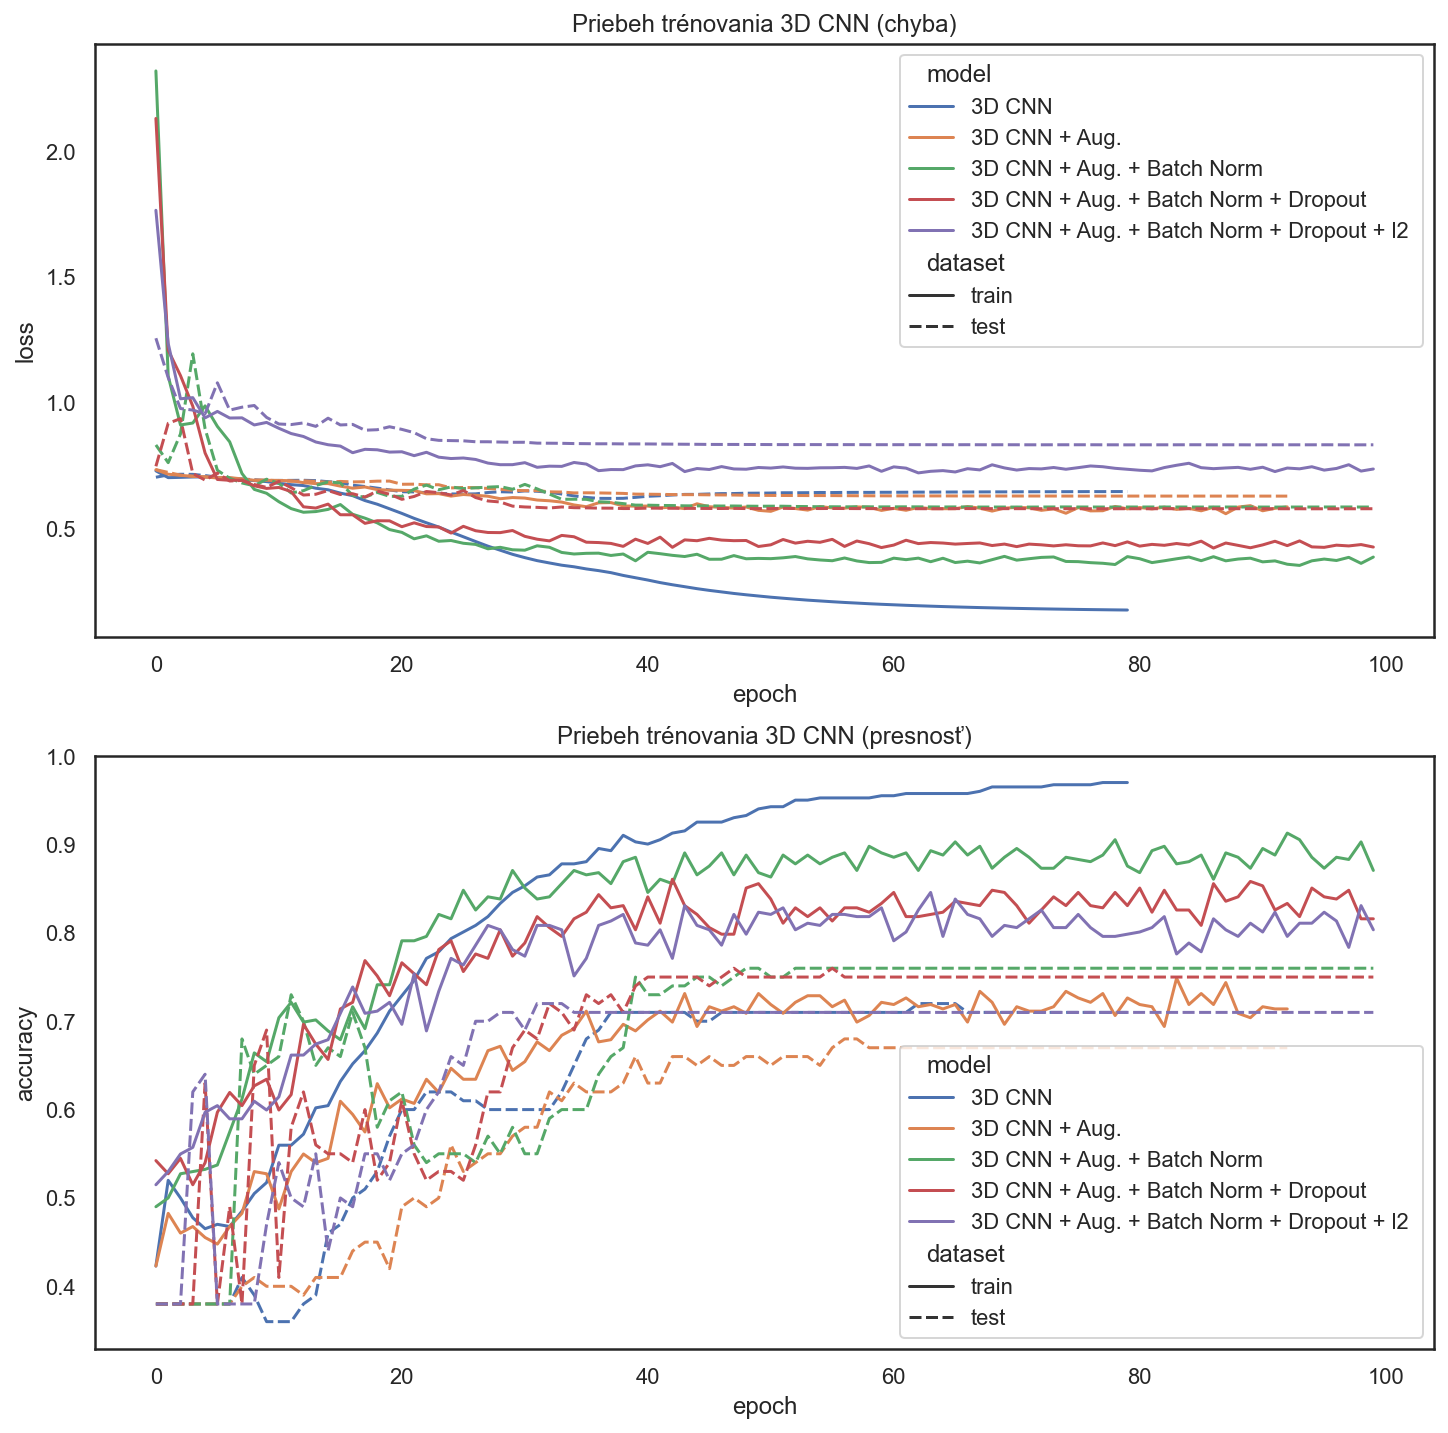
\includegraphics[width=14cm]{assets/images/3d_cnn_training.png}
    \caption{Priebeh trénovania 3D konvolučnej neurónovej siete, čím viac sme pridali regularizácie (l2 alebo dropout) tým sme dosiahli horšie výsledky. Po pridaní augmentácií sa úspešnosť modelu zhoršila, avšak následne sa už iba zlepšovala.}
    \label{fig:3d_cnn_training}
\end{figure}

\begin{figure}[h!]
    \centering
    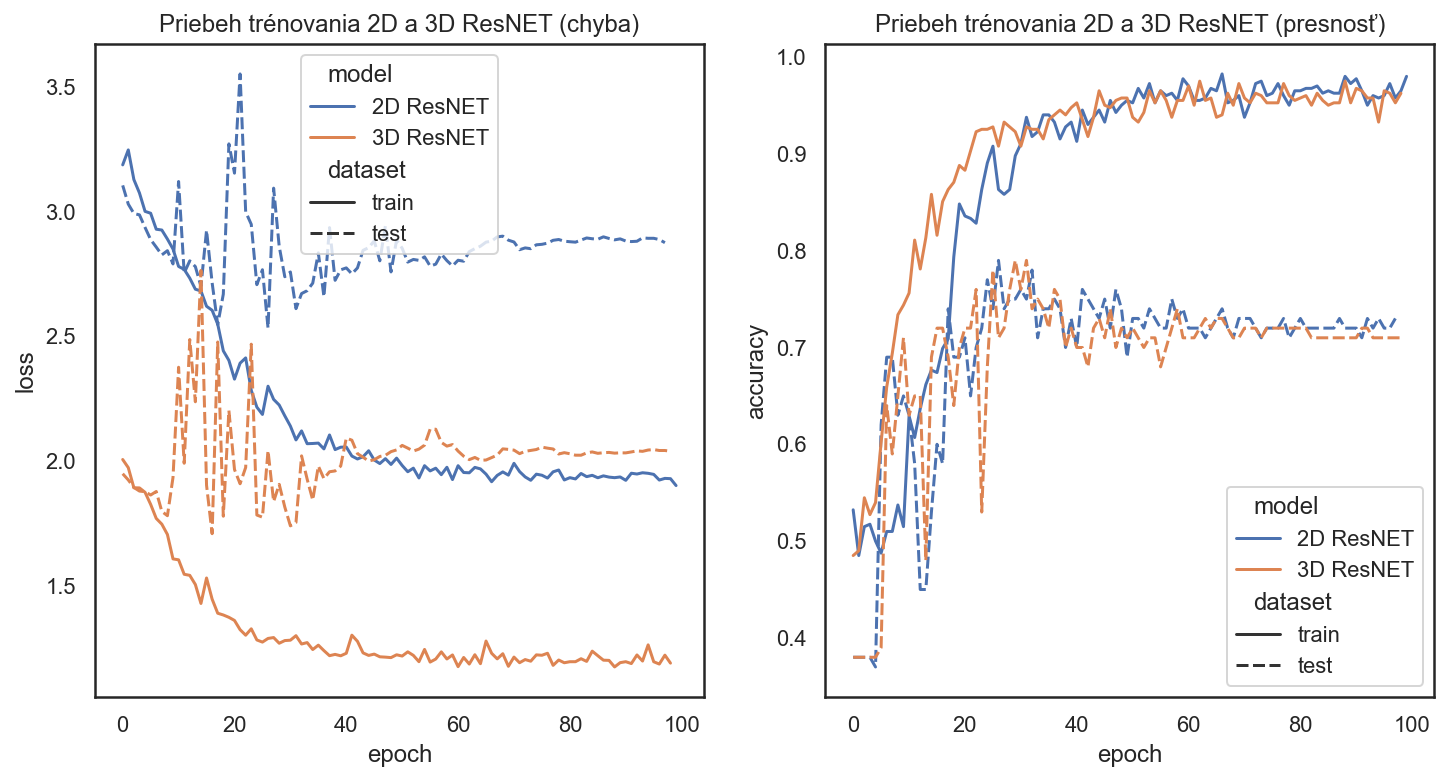
\includegraphics[width=14cm]{assets/images/2d_3d_res_net_training.png}
    \caption{Priebeh trénovania 2D a 3D ResNet neurónovej siete. V oboch prípadoch sme použili dropout aj regularizáciu. Od približne 30-tej epochy sa neurónová sieť začala pretrénovávať, aj napriek regularizácii. Ako vylepšenie je možné skúsiť silnesjšiu regularizáciu (väčšiu hodnotu l2 a dropout), ak ani to nepomôže, je možné, že architektúra je príliš komplexná náš problém (neurónová sieť je príliš hlboká). Môžeme ďalej skúsiť odstrániť jednu plne prepojenú vrstvu alebo znížiť počet neurónov v týchto vrstvách.}
    \label{fig:2d_3d_res_net_training}
\end{figure}

\section{Záver}

V tejto kapitole sme opísali ako sme implementovali nami navrhovanú metódu a spôsob jej overenie. Opísali sme implemetáciu kľúčových prvkov (generovanie masiek a vytvorenie tepelnej mapy) navrhovanej metódy RISEI a jej hyper parametre. Rovnako sme opísali aj implementáciu neurónovej siete, architektúru, spôsob trénovania a použitú dátovú sadu. Metódu RISEI sa nám podarilo implementovať a je ich možné použiť v experimentoch. Podarilo sa nám natrénovať niekoľko architektúr neurónových sietí, pričom sme indetifikovali možné príčiny (a navrhli k nim riešenia) výsledkov, ktoré dosahujú. Každopádne výsledky považujeme za postačujúce pre prvé experimenty navrhovanej metódy RISEI.
